\chapter{FLOCKING ALGORITHM}\label{chap3}

% introduction
%\section{Introduction}
The behavior seen in social animals like birds and fishes is called \textit{flocking}. Flocking algorithms are used to simulate this social behavior by following a set of simple rules. These rules were introduced by the pioneer of flocking Craig Reynolds\cite{craig1}. The three main rules or steering behaviors are: separation, alignment, and cohesion. This chapter discusses the different behaviors implemented in our code, which include the three main steering behaviors, along with a three more behaviors.

% 3 steering behaviors
\section{Three Main Steering Behaviors}
Boid evolution is subject to several behavior rules. To each rule, we associate a velocity vector that will direct the movement of the boid. These velocity vectors are added together, each subject to a scalar weight. More generally, given rule $i$, and a scalar weight $w_i$, the boid will move in the direction of the velocity, 
$$
v = \sum_i w_i v_i
$$
%The steering behaviors are velocity vectors, they have direction and magnitude. 
Each behavior is evaluated at each time step for each boid.

% separation
\subsection{Separation}\label{separationsection}
\textit{Separation} can be described as the steering velocity that maintains each entity of the flock separated by at least a minimum determined distance. Craig Reynolds first called this rule \textit{collision avoidance} to indicate that boids tried to avoid colliding with nearby flockmates. Later on, the rule was changed to \textit{separation}. This steering behavior prevents excessive crowding of boids. Figure~\ref{separationPDF} shows that only flockmates within a certain radius $R_{sep}$ are considered when evaluating this behavior. The red vector is the resulting steering velocity.

% separation figure
\begin{figure}[htbp]
\begin{center}
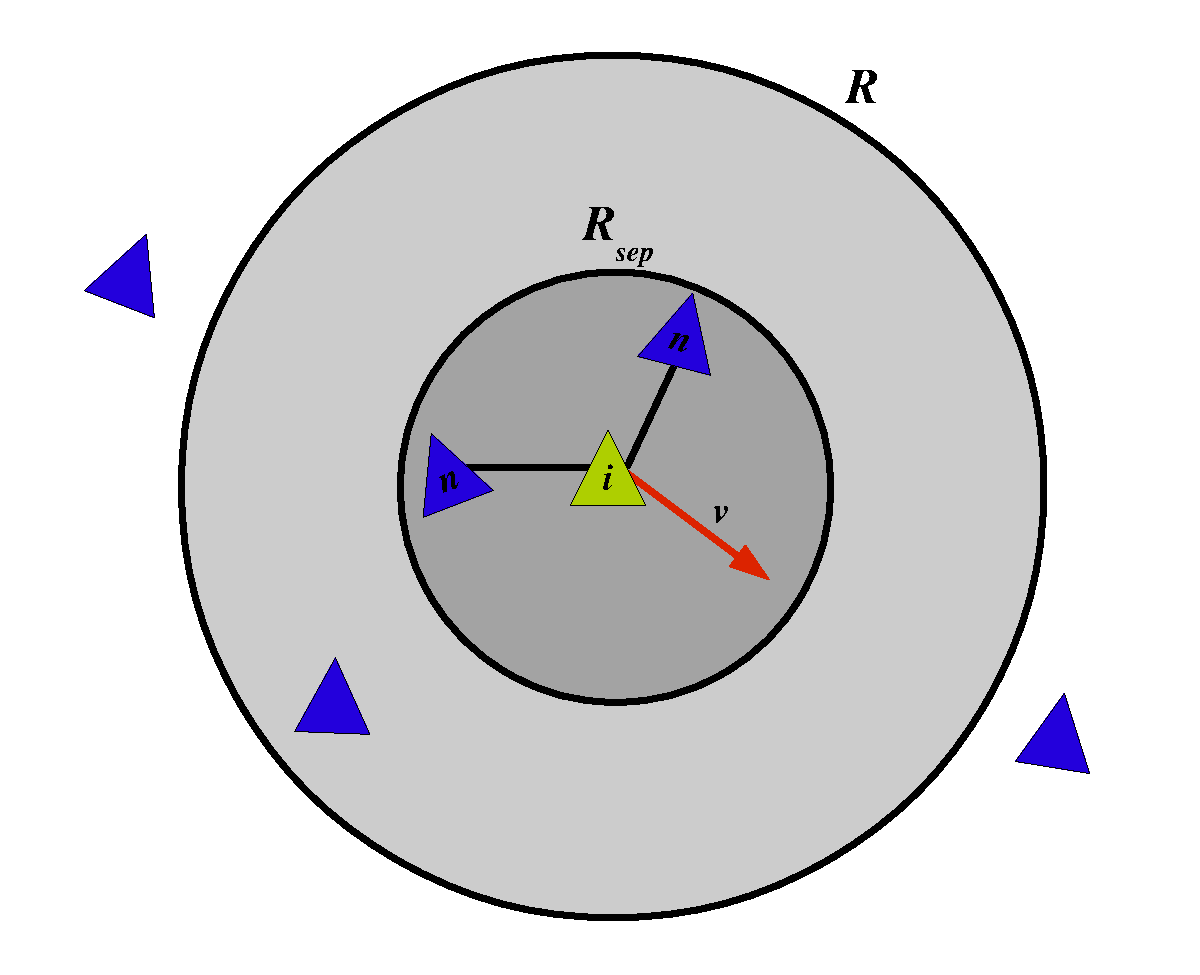
\includegraphics[scale=0.6]{figures/separation.pdf}
\caption{Separation steering velocity: the outer circle is the neighborhood of boid $i$, the inner circle is the minimum distance neighborhood, \textit{separation} steers boid $i$ away/near the neighboring boids until a minimum distance between them is met}
\label{separationPDF}
\end{center}
\end{figure}

Separation is a repulsive velocity. The mathematical expression that was implemented is showed in equation~\ref{separationEquation}.

% separation equation
\begin{equation}
\label{separationEquation}
Separation =\frac{1}{M} \sum_{n=1}^{M} \frac{p_i - p_n}{d(p_i,p_n)},
\end{equation}
where $M$ is the number of boids within the minimum distance from boid $i$, $p_i$ is the position of boid $i$, and $d(p_i,p_n)$ is the distance between boids $i$ and boid $n$.

%Only neighbors that are within the minimum separation distance are considered. The difference between the positions of boid $i$ and boid $n$ is divided by the distance between boid $i$ and boid $n$ are summed. Then, the sum is divided by the number of boids that were within the minimum distance. The resulting vector corresponds to the \textit{separation} steer of boid $i$ with respect to their nearest flockmates. 

The separation velocity of boid $i$ is a linear combination of unit vectors pointing toward nearest neighbors. Thus each neighboring boid exerts equal influence on boid $i$, with only direction changing. 

% alignment
\subsection{Alignment}
\textit{Alignment} is the steering behavior through which boids try to align themselves with their neighbors. Reynolds initially called this behavior \textit{velocity matching}, later the name was changed to \textit{alignment}. This behavior also prevents crowding. According to this rule, each boid would \textit{align} its heading with the average heading of their flockmates. Figure~\ref{alignmentPDF} shows the corrective steering velocity vector in red.

% alignment figure
\begin{figure}[htbp]
\begin{center}
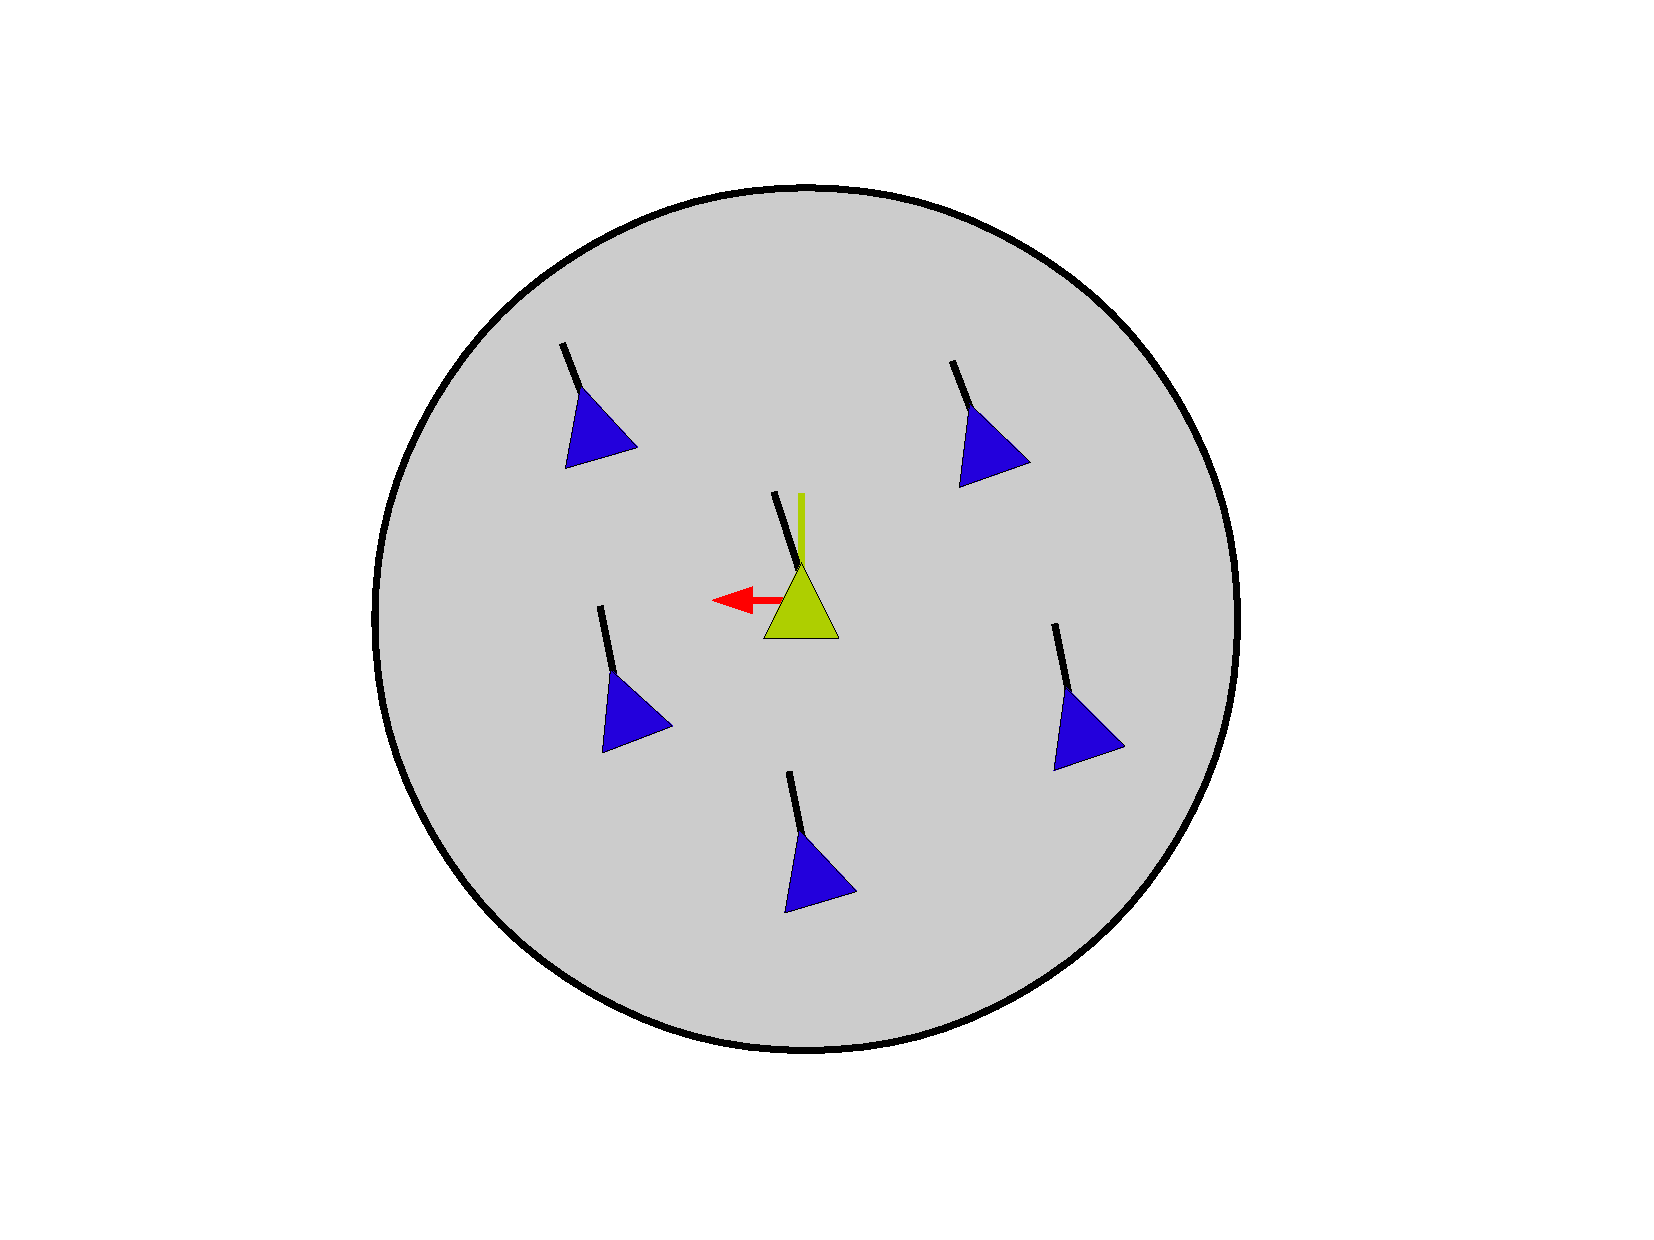
\includegraphics[scale=0.6]{figures/alignment.pdf}
\caption{Alignment steering velocity: the circle is the neighborhood of boid $i$, \textit{alignment} match the heading and speed of boid $i$ with respect to their neighbors}
\label{alignmentPDF}
\end{center}
\end{figure}

\textit{Alignment} is also calculated in the local neighborhood of each boid. This steering behavior was computed using equation~\ref{alignmentEquation}.

% alignment equation
\begin{equation}
\label{alignmentEquation}
Alignment = \left[  \frac{1}{N} \sum_{n=1}^{N} v_n \right ] - v_i
\end{equation}
where $N$ is the number of boids within the search radius centered at boid $i$. This radius $R$ is larger than $R_{sep}$ and $v_n$ is the velocity of boid $n$. The \textit{alignment} corrective velocity is computed by calculating the desired velocity which is the center of mass with respect to the velocities, and then subtracting off the velocity of boid $i$.

% cohesion
\subsection{Cohesion}
\textit{Cohesion} is responsible for steering boids towards the center of the flock. When Reynolds introduced his \textit{Boids} model, he called this behavior \textit{flock centering} and defined it as \textit{the attempt to stay close to nearby objects}. The definition was kept while the name of the rule changed to \textit{cohesion}. This behavior makes each boid attracted to the center of the flock. In our case each boid is attracted to the center of mass of its local neighborhood. Figure~\ref{cohesionPDF} shows the \textit{cohesion} steering velocity in red.

% cohesion figure
\begin{figure}[htbp]
\begin{center}
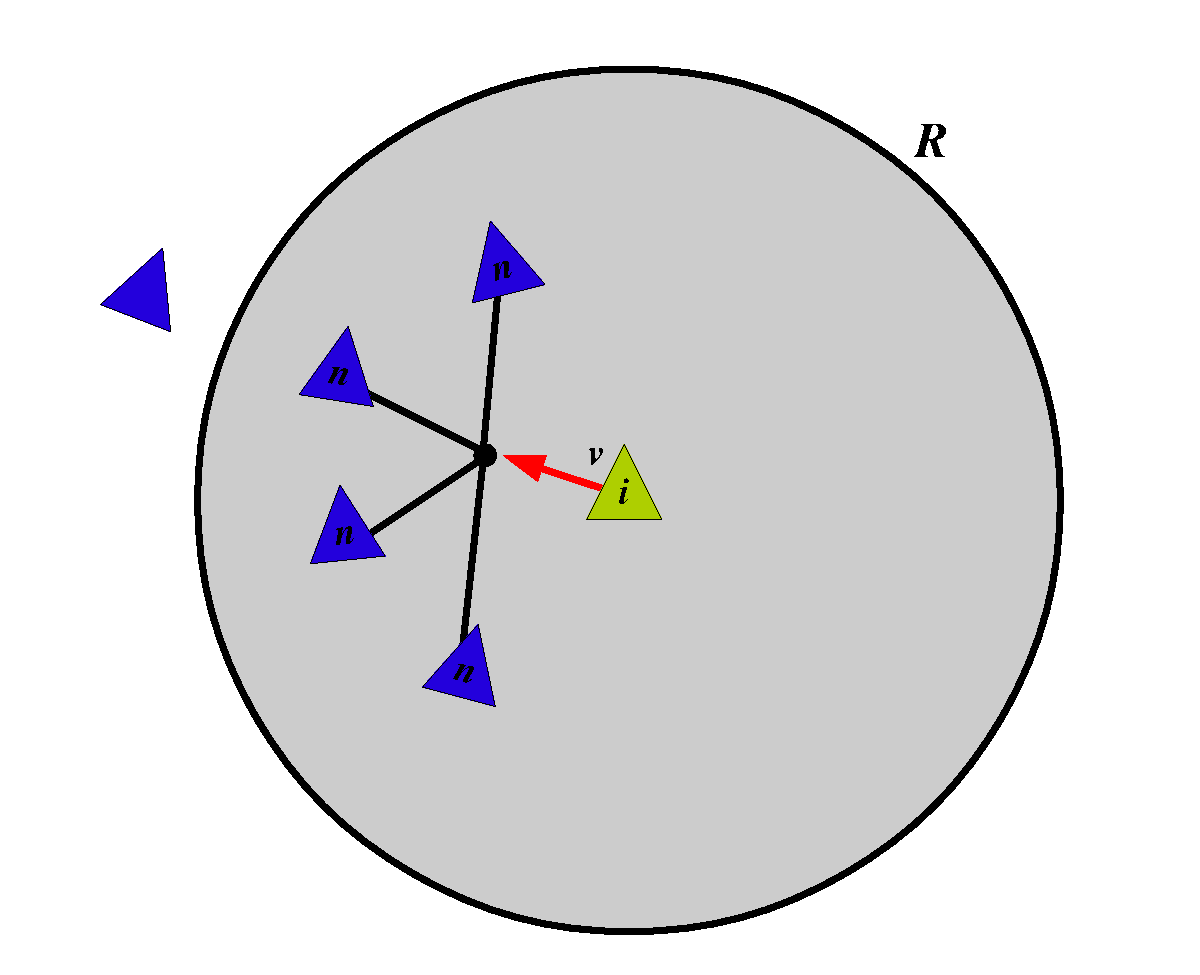
\includegraphics[scale=0.6]{figures/cohesion.pdf}
\caption{Cohesion steering velocity: the circle is the neighborhood of boid $i$, \textit{cohesion} steers boid $i$ towards the center of its local neighborhood}
\label{cohesionPDF}
\end{center}
\end{figure}

The formula used for \textit{cohesion} is very similar to the formula used for \textit{alignment}, the only difference is that \textit{cohesion} uses the positions of the boids while \textit{alignment} uses the boid velocities (Equation~\ref{cohesionEquation}),

% cohesion equation
\begin{equation}
\label{cohesionEquation}
Cohesion = \left[  \frac{1}{N} \sum_{n=1}^{N} p_n \right ] - p_i, 
\end{equation}
where $N$ is the number of boids in the local neighborhood of boid $i$. $p_n$ is the position of the flockmate $n$. The direction of movement for boid $i$ is towards the center of mass determined from the boids in its neighborhood. 

% other behaviors
\section{Other Steering Behaviors}\label{otherbehaviors}
Besides the three main steering behaviors just discussed, there have been many more steering velocities that have been considered. In this section, we discuss three additional behaviors that we have implemented: \textit{goal}, \textit{avoid}, and \textit{follow the leader}.

% goal
\subsection{Goal}
\textit{Goal} is the steering behavior that attracts boids to a specific location in global space. This location is static. Figure~\ref{seekfleePDF} shows the action taken when approaching or avoiding the target. The red vector shows the direction taken by the boid towards the \textit{goal}, while the blue vector illustrates the boid would take to avoid the goal. We discuss this further in the next Section. The gray vector to the right of the boid is the desired velocity, while the dotted line is the actual path taken by the boid.

% seek and flee figure
\begin{figure}[htbp]
\begin{center}
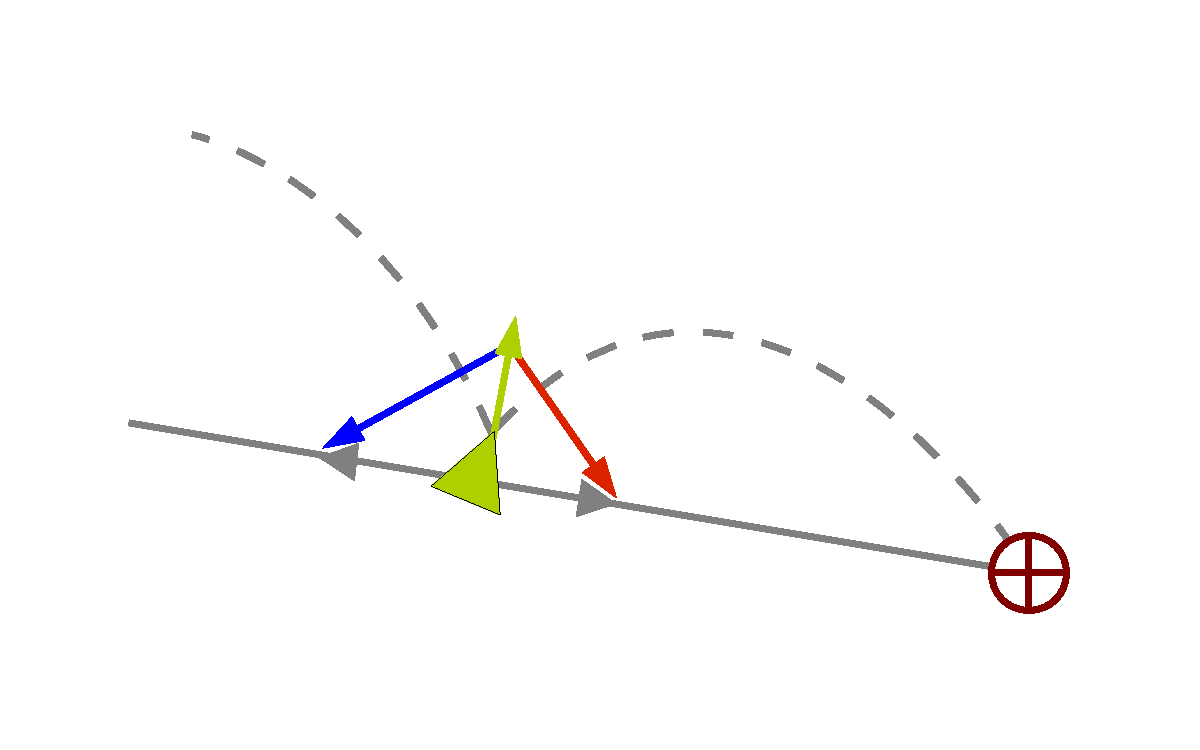
\includegraphics[scale=0.75]{figures/seekANDflee.pdf}
\caption{Goal and Avoid behaviors: boid $i$ would approach the target when subject to a \textit{goal} behavior, or would steer clear of the target when following the \textit{avoid} behavior }
\label{seekfleePDF}
\end{center}
\end{figure}

The \textit{Goal} behavior adjusts the boid's velocity in such a way that it is aligned towards the target. \textit{How it is computed?} Since the target is static, the position of the boid is subtracted from the position of the target, the resulting vector is normalized and multiplied by the maximum speed of the boid. To get the steering vector, subtract the current velocity vector from the desired velocity vector. More succinctly, 

% goal equation
\begin{equation}
\label{goalEquation}
Goal = \left[\frac{(p_t - p_i)}{dist(p_t,p_i)} * max_{speed} \right] - v_i
\end{equation}
where $p_i$ and $v_i$ are the position and velocity of boid $i$, respectively, and $p_t$ is the position of the target. This rule causes the boid to keep approaching the goal, without necessarily ever reaching it, somewhat akin to a moth buzzing around a light bulb.

% avoid
\subsection{Avoid}
\textit{Avoidance} refers to a boid steering away from a static target in the global space. The approach is similar to the \textit{goal} steering with the difference that the desired velocity points in the opposite direction. Figure~\ref{seekfleePDF} depicts the steering vector in blue and the desired velocity in gray (at the left side of the boid). Equation~\ref{avoidEquation} shows the mathematical formula for \textit{avoid}:

% avoid equation
\begin{equation}
\label{avoidEquation}
Avoid = -\left[\frac{(p_t - p_i)}{dist(p_t,p_i)} * max_{speed} \right] - v_i
\end{equation}

In this formula $\frac{(p_t - p_i)}{dist(p_t,p_i)}$ is referred to as the desired velocity. For the \textit{avoid} behavior there is a negative sign preceding the desired velocity to indicate that it points in a direction opposite to the velocity in \textit{goal} behavior.

% leader following
\subsection{Follow the Leader}
The \textit{Follow the Leader} behavior is when there is a boid in charge of the flock, called \textit{leader}, and the rest of the boids in the flock become \textit{followers}. This is one of the many complex behaviors that a flock can exhibit as a whole. Followers come in slightly behind the leader using "it" as a target, while the leader targets an specific location in the global space.

% leader following figure
\begin{figure}[htbp]
\begin{center}
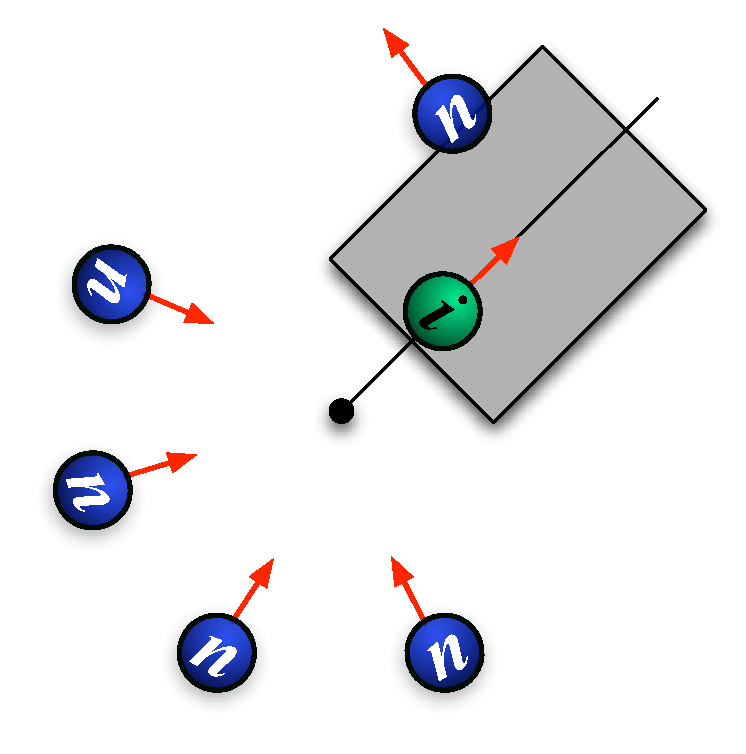
\includegraphics[scale=0.75]{figures/leaderFollowing.pdf}
\caption{Leader Following behavior: the followers follow the leader by approaching a point slightly behind the leader. If a follower find itself in a rectangular area in front of the leader it will move out of the leader's way.}
\label{leaderPDF}
\end{center}
\end{figure}

Generally, the followers tend to stay close to the leader while staying out of its path, as seen in Figure~\ref{leaderPDF}. If a follower is within the rectangular region ahead of the leader it distances itself, clearing a path for the leader to move freely without worry of collision. The leader's movement is  based on Equation~\ref{goalEquation} where $p_t$ is the leader's target position within the global space.The followers that are outside the rectangular region will approach a point slightly behind the leader, also governed by Equation~\ref{goalEquation}.

% combining behaviors
\section{Combining the Steering Behaviors}
Each of the steering behaviors discussed above returns a velocity vector. These velocities are combined linearly to produce a final boid velocity. In this Section we use only \textit{separation}, \textit{alignment}, and \textit{cohesion} to simplify the length of the equations. The strength of each velocity contribution is controlled by a separate weight constant, specified by the user: 

%velocity contribution is 
%The question that nwo  arises is \textit{how to combine the behaviors in order to move the boids?}. Each steering force multiplied by a respective weight\footnote{Weights are given by the user, they are not constant values assigned by us.}. For example, combining \textit{separation}, \textit{alignment}, and \textit{cohesion} is done by using Equation~\ref{combine}. Each behavior is multiplied by its constant weight, then they are added to get the final velocity vector.
%

% combine equation
\begin{equation}
\label{combine}
velocity = C_S Separation  + C_A Alignment  + C_C Cohesion 
\end{equation}

%\mmy{I do not see avoidance and the other behaviors you implemented}
%The \textit{new} velocity is just the velocity of Equation~\ref{combine} plus the current velocity. 
A first order Euler integration method is used  to calculate the \textit{new} position of each boid: 

% integrate equation
\begin{align}
\label{integrate}
p_i^{k=1} = p_i^k + dt~ v_i
\end{align}
where $p_i^{k+1}$ is the position of boid $i$ at step $k+1$, $v_i$ is the velocity of the boid, and $dt$ is the integration time step. 

The various velocities are recomputed and the boid positions are updated at every time step. 

% algorithms
\section{Algorithms}

In this Section, we present three algorithms. The first algorithm computes the different steering rules. The second algorithm combines the rules and updates the boid positions, and the third algorithm updates the FLOCK boids system at each frame of the simulation. 

The following Algorithm presents the GPU implementation of each of the steering rules. To save time, one only computes the rules with non-zero weights. 

% flocking algorithm
\begin{algorithm}
\caption{Flocking algorithm to follow Separation, Alignment, Cohesion, Goal, and Avoid steering behaviors}
\label{flockingAlgorithm}
\begin{algorithmic}
\FOR {each neighbor $j$ of boid $i$}
	\IF{dist($pos_i$, $pos_j$) $<=$ searching radius}
	\STATE flockmates++
		\IF{$w_{sep} > 0$}
			\IF{dist($pos_i$, $pos_j$) $<=$ minimum distance}
				\STATE nearestFlockmates++
				\STATE s = $pos_i$ - $pos_j$ 
				\STATE s /= dist($pos_i$, $pos_j$) 
				\STATE separation += s
			\ENDIF
		\ENDIF
		\IF{$w_{align} > 0$}
			\STATE alignment += $vel_j$
		\ENDIF
		\IF{$w_{coh} > 0$}
			\STATE cohesion += $pos_j$
		\ENDIF
	\ENDIF
\ENDFOR
\IF{$w_{sep} > 0$ \&\& nearestFlockmates $> 0$}
	\STATE separation /= nearestFlockmates
\ENDIF
\IF{$w_{align} > 0$ \&\& flockmates $> 0$}
	\STATE alignment /=  flockmates
	\STATE alignment -= $vel_i$
\ENDIF
\IF{$w_{coh} > 0$ \&\& flockmates $> 0$}
	\STATE cohesiont /=  flockmates
	\STATE cohesion -= $pos_i$
\ENDIF
\IF{$w_{goal} > 0$}
	\STATE $pos_t$ = target
	\STATE desiredVel = (normalize($pos_t - pos_i$) * $max_{speed}$) / dist($pos_t, pos_i$) 
	\STATE goal = desiredVel - $vel_i$
\ENDIF
\IF{$w_{avoid} > 0$}
	\STATE $pos_t$ = target
	\STATE desiredVel = -(normalize($pos_t - pos_i$) * $max_{speed}$) / dist($pos_t, pos_i$) 
	\STATE avoid = desiredVel - $vel_i$
\ENDIF

\end{algorithmic}
\end{algorithm}

In the Algorithm~\ref{flockingAlgorithm}, each rule is computed sequentially for each boid. The iterative loop is over the flockmates of boid $i$. First we determine (and count) the flockmates in the neighborhood covered by the searching radius, which are input into rules \textit{cohesion} and \textit{alignment}. A similar approach was taken for the CPU implementation of Algorithm~\ref{flockingAlgorithm}.

% combine and integrate
\begin{algorithm}
\caption{Combine, integrate and check the boundaries}
\label{combineAlgorithm}
\begin{algorithmic}
\STATE $vel_{rule_j}$  = $rule_j$ * $w_{rule_j}$ 
\STATE $vel_i^{k+1}$ = $vel_i^k$ + $vel_{rule_1}$ + ... + $vel_{rule_n}$
\IF{length($vel_i^{k+1}$) $>$ $max_{speed}$}
	\STATE $vel_i^{k+1}$ = normalize($vel_i^{k+1}$) * $max_{speed}$
\ENDIF  
\STATE (Optional) Add an imposed velocity field to the current velocity.
\STATE $pos_i^{k+1}$ = $pos_i^{k}$ + $dt$ * $vel_i^{k+1}$
\STATE Apply periodic boundary conditions to the \textit{new} position.
\end{algorithmic}
\end{algorithm}

Algorithm~\ref{combineAlgorithm} presents the steps necessary to update the boid's position at each time step. For each $j$ rule, the respective velocity is computed. By adding the velocities of each rule and the current velocity, the final velocity vector of boid $i$ at time step $k+1$ is obtained. First order, Euler integration is done to calculate the positions. Since flocking is an overall behavior we are not concern on getting very accuracy positions. A first order algorithm is enough. We would like to maintain the boid's density in our system, that is why we applied periodic boundary conditions to the positions to the boids.
 
% update
\begin{algorithm}
\caption{Update of each frame of the simulation}
\label{updateAlgorithm}
\begin{algorithmic}
\STATE Create a FLOCK boids system.
\FOR {each frame}
\STATE Do the nearest neighbor search.
\STATE Compute that rule.
\STATE Integrate over time.
\STATE Render the new position.
\ENDFOR
\end{algorithmic}
\end{algorithm}

The last algorithm presented is Algorithm~\ref{updateAlgorithm} which is a simplified version of 
the \texttt{updateGPU()} function (Section~\ref{flocksection}). First a FLOCK boids system is created. The boids then enter into a continuous loop that is broken when the simulation ends. 
